\documentclass[letterpaper,11pt]{article}

% Soporte para los acentos.
\usepackage[utf8]{inputenc}
\usepackage[T1]{fontenc}
% Idioma español.
\usepackage[spanish,mexico, es-tabla]{babel}
% Soporte de símbolos adicionales (matemáticas)
\usepackage{multirow}
\usepackage{amsmath}
\usepackage{amssymb}
\usepackage{amsthm}
\usepackage{amsfonts}
\usepackage{mathtools}
\usepackage{latexsym}
\usepackage{enumerate}
\usepackage{ragged2e}
\usepackage{listings}
\usepackage{xcolor}
\usepackage{graphicx}
\usepackage{hyperref}
% Modificamos los márgenes del documento.                                       %
\usepackage[lmargin=2cm,rmargin=2cm,top=2cm,bottom=2cm]{geometry}

\definecolor{codegreen}{rgb}{0,0.6,0}
\definecolor{codegray}{rgb}{0.5,0.5,0.5}
\definecolor{codepurple}{rgb}{0.58,0,0.82}
\definecolor{backcolour}{rgb}{0.95,0.95,0.92}

\lstdefinestyle{mystyle}{
    backgroundcolor=\color{backcolour},   
    commentstyle=\color{codegreen},
    keywordstyle=\color{magenta},
    numberstyle=\tiny\color{codegray},
    stringstyle=\color{codepurple},
    basicstyle=\ttfamily\footnotesize,
    breakatwhitespace=false,         
    breaklines=true,                 
    captionpos=b,                    
    keepspaces=true,                 
    numbers=left,                    
    numbersep=5pt,                  
    showspaces=false,                
    showstringspaces=false,
    showtabs=false,                  
    tabsize=2
}

\lstset{style=mystyle}

\title{Facultad de Ciencias, UNAM \\ Redes Neuronales \\ Tarea 5}
\author{Rubí Rojas Tania Michelle}
\date{1 de junio de 2020}

\begin{document}
\maketitle

\begin{enumerate}
    % Ejercicio 1.
    \item Construye una red neuronal convolucional para detectar las imágenes
    en el \textit{dataset} de perros y gatos. 

    \textsc{Solución:} Primero, descomprimimos cada uno de nuestros archivos 
    \textit{.zip} y los almacenamos en una carpeta llamada \textit{dataset}:
    \begin{lstlisting}[language=Python]
    from zipfile import ZipFile

    # Le hacemos un unzip a nuestro conjunto de entrenamiento.
    with ZipFile('dataset/train_dogscats.zip', 'r') as zipObj:
        zipObj.extractall('dataset')

    # Le hacemos un unzip a nuestro conjunto de prueba.
    with ZipFile('dataset/test_dogscats.zip', 'r') as zipObj:
        zipObj.extractall('dataset')
    \end{lstlisting}

    Creamos un \textit{dataframe} con cada una de las imágenes dentro de la 
    carpeta \textit{train}. Como el nombre de cada imagen nos indica si el 
    animalito es un perro o es un gato, extraeremos esa información.
    \begin{lstlisting}[language=Python]
    import os
    import pandas as pd

    nombres = os.listdir("dataset/train")
    categorias = []
    for nombre in nombres:
        animal = nombre.split('.')[0] # Obtenemos el nombre del animalito.
        if(animal == 'dog'):
            categorias.append(1)
        else:
            categorias.append(0)
            
    data_frame = pd.DataFrame({'nombre'   : nombres,
                            'categoria': categorias
                            })

    # Visualizamos el dataframe con 10 archivos.
    data_frame.head(10)
    \end{lstlisting}

    \begin{figure}[ht]
        \centering
        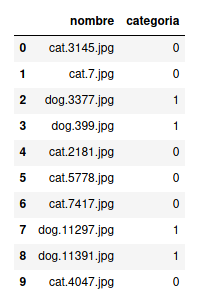
\includegraphics[width=0.3\textwidth]{./imagenes/dataframe.png}
    \end{figure} 

    \newpage
    Así, tenemos un \textit{dataframe} con cada una de las imágenes y sus 
    respectivas etiquetas.

    Ahora, dividimos nuestro conjunto de datos en entrenamiento y prueba.
    \begin{lstlisting}[language=Python]
    from sklearn.model_selection import train_test_split

    # Convertimos la variable "categoria" en gato o perro.
    data_frame["categoria"] = data_frame["categoria"].replace({0:'gato', 
                                                               1:'perro'
                                                              })

    # Dividimos nuestro conjunto de datos con un split del 75-25 para 
    # entrenamiento y prueba.
    X_train, X_test = train_test_split(data_frame, 
                                       test_size    = 0.25, 
                                       random_state = 42)

    # Reestablecemos los indices de nuestros datos.
    X_train = X_train.reset_index(drop = True)
    X_test = X_test.reset_index(drop = True)

    # Obtenemos su respectivo numero de columnas. 
    total_train = X_train.shape[0]
    total_test = X_test.shape[0]
    \end{lstlisting}

    \begin{lstlisting}[language=Python]
    from keras.preprocessing.image import ImageDataGenerator, load_img

    # Modificamos las imagenes para poder obtener mas datos con los que 
    # entrenar.
    datos_train = ImageDataGenerator(rotation_range     = 15,
                                     rescale            = 1./255, # Normalizamos.
                                     shear_range        = 0.1,
                                     zoom_range         = 0.2,
                                     horizontal_flip    = True,
                                     width_shift_range  = 0.1,
                                     height_shift_range = 0.1
                                    )



    # Generamos las imagenes de entrenamiento.
    generador_train = datos_train.flow_from_dataframe(X_train,
                                                      "dataset/train/",
                                                      x_col       = 'nombre',
                                                      y_col       = 'categoria',
                                                      target_size = (128, 128),
                                                      class_mode  = 'categorical',
                                                      batch_size  = 15
                                                     )

    # Generamos las imagenes de prueba.
    datos_test = ImageDataGenerator(rescale = 1./255)
    generador_test = datos_test.flow_from_dataframe(X_test, 
                                                    "dataset/train/", 
                                                    x_col       = 'nombre',
                                                    y_col       = 'categoria',
                                                    target_size = (128, 128),
                                                    class_mode  ='categorical',
                                                    batch_size  = 15
                                                   )
    \end{lstlisting}

    \begin{verbatim}
        Found 18750 validated image filenames belonging to 2 classes.
        Found 6250 validated image filenames belonging to 2 classes.

    \end{verbatim}

    Luego, diseñamos el modelo de nuestra red convolucional.
    \begin{lstlisting}[language=Python]
    from keras.models import Sequential
    from keras.layers import Convolution2D, MaxPooling2D, Dropout, Flatten, 
                             Dense, Activation, BatchNormalization

    model = Sequential()

    # Primer capa. 
    model.add(Convolution2D(32, (3, 3), activation = 'relu', 
                            input_shape = (128, 128, 3)))
    model.add(BatchNormalization())
    model.add(MaxPooling2D(pool_size = (2, 2)))
    model.add(Dropout(0.25))

    # Segunda capa.
    model.add(Convolution2D(64, (3, 3), activation='relu'))
    model.add(BatchNormalization())
    model.add(MaxPooling2D(pool_size = (2, 2)))
    model.add(Dropout(0.25))

    # Tercer capa.
    model.add(Convolution2D(128, (3, 3), activation = 'relu'))
    model.add(BatchNormalization())
    model.add(MaxPooling2D(pool_size = (2, 2)))
    model.add(Dropout(0.25))

    # Cuarta Capa: fully-connected. 
    model.add(Flatten())
    model.add(Dense(512, activation='relu'))
    model.add(BatchNormalization())
    model.add(Dropout(0.5))

    # Clasificador Softmax.
    model.add(Dense(2, activation = 'softmax'))
    \end{lstlisting}

    Analizamos el modelo.
    \begin{lstlisting}[language=Python]
        model.summary()
    \end{lstlisting}

    \begin{figure}[ht]
        \centering
        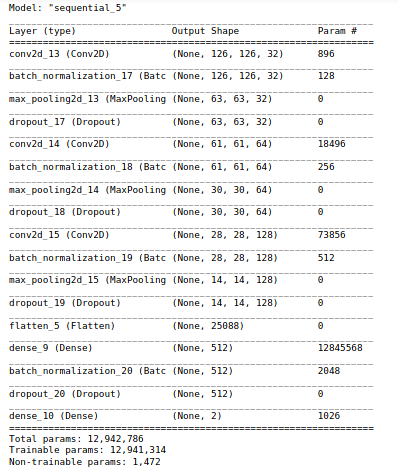
\includegraphics[width=0.45\textwidth]{./imagenes/modelo.png}
    \end{figure} 

    Finalmente, lo compilamos. 
    \begin{lstlisting}[language=Python]
    model.compile(loss      = 'categorical_crossentropy',
                  optimizer = 'rmsprop',
                  metrics   = ['accuracy'])
    \end{lstlisting}

    Ahora, toca el turno del entrenamiento. Notemos que \textit{EarlyStopping}
    lo utilizamos para evitar el exceso de ajuste (detenemos el aprendizaje 
    después de que $epochs = 10$ y el valor de val\_loss no haya disminuido) y 
    \textit{ReduceLROPlateau} lo utilizamos para manejar la tasa de aprendizaje 
    de la red (la reducimos cuando la precisión no aumenta en $2$ steps). 
    \begin{lstlisting}[language=Python]
    from keras.callbacks import EarlyStopping, ReduceLROnPlateau

    H = model.fit(generador_train, 
                  epochs           = 10,
                  validation_data  = generador_test,
                  validation_steps = total_test // 15,
                  steps_per_epoch  = total_train // 15,
                  callbacks        = [EarlyStopping(patience = 10), 
                                      ReduceLROnPlateau(monitor  = 'val_accuracy',
                                                    patience = 2, verbose = 1,
                                                    factor = 0.5,min_lr = 0.00001)]
                 )
    \end{lstlisting}

    \begin{figure}[ht]
        \centering
        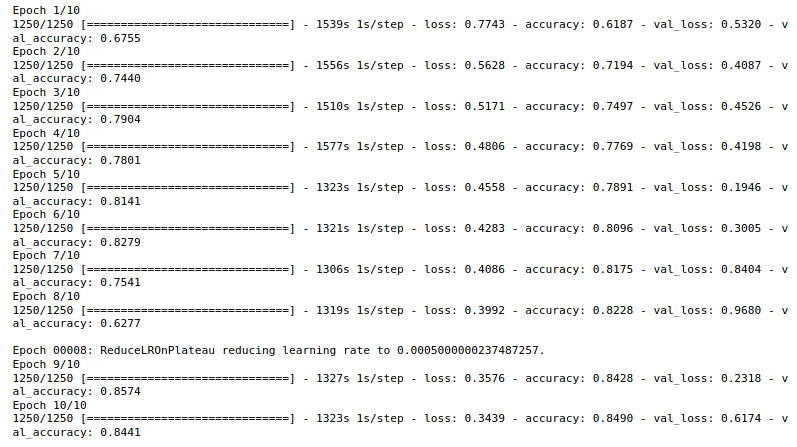
\includegraphics[width=0.99\textwidth]{./imagenes/epochs.png}
    \end{figure} 

    Evaluamos qué tan bien le fue con nuestro conjunto de prueba.
    \begin{lstlisting}[language=Python]
    score = model.evaluate(generador_train, steps = len(generador_train))
    \end{lstlisting}

    \begin{verbatim}
        1250/1250 [==============================] - 330s 264ms/step
    \end{verbatim}
    
    \begin{lstlisting}[language=Python]
    print("Score {}".format(score))
    \end{lstlisting}

    \begin{verbatim}
        Score [0.23800379037857056, 0.8423466682434082]
    \end{verbatim}

    Obtenemos un $0.84\%$ de precisión.
    \begin{figure}[ht]
        \centering
        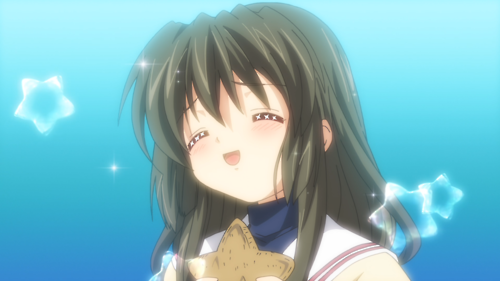
\includegraphics[width=0.5\textwidth]{./imagenes/fuko.png}
    \end{figure} 

    % Ejercicio 2.
    \item ¿Qué arquitectura diseñaste?
    
    \textsc{Solución:} Diseñamos una \textit{red neuronal convolucional} con 
    la siguiente estructura
    \begin{itemize}
        \item Capa Uno

        Tiene una capa convolucional de $3 \times 3$ (sin paddings, aprendemos
        un total de $32$ filtros, utilizamos la función de activación 
        \textit{ReLU} e indicamos el tamaño de las imágenes), una capa de Batch 
        Normalization (para aumentar la estabilidad de la red neuronal), una 
        capa de MaxPooling de $2 \times 2$ y una capa de Dropout de $0.25$.  

        \item Capa Dos

        Tiene una capa convolucional de $3 \times 3$ (sin paddings, aprendemos 
        un total de $64$ filtros y utilizamos la función de activación 
        \textit{ReLU}), una capa de Batch Normalization (para aumentar la 
        estabilidad de la red neuronal), una capa de MaxPooling de $2 \times 2$
        y una capa de Dropout de $0.25$. 

        \item Capa Tres
        
        Tiene una capa convolucional de $3 \times 3$ (sin paddings, aprendemos 
        un total de $128$ filtros y utilizamos la función de activación 
        \textit{ReLU}), una capa de Batch Normalization (para aumentar la 
        estabilidad de la red neuronal), una capa de MaxPooling de $2 \times 2$
        y una capa de Dropout de $0.25$.

        \item Cuarta Capa: fully-connected. 
        
        Añadimos una única capa fully-connected con $512$ nodos (cuya función de 
        activación es \textit{ReLU}) a nuestra red convolucional. 

        \item Clasificador Softmax.

        Añadimos el clasificador Softmax (vamos a tener dos clases: perros y 
        gatos). La salida de esta capa son los valores propios de predicción. 
    \end{itemize}

    % Ejercicio 3.
    \item Haz las gráficas de pérdida y de precisión tanto para el entrenamiento
    como para la validación y preséntalas.

    \textsc{Solución:} 
    \begin{itemize}
        \item Pérdida
        \begin{lstlisting}[language=Python]
        import matplotlib.pyplot as plt

        plt.plot(H.history['loss'])
        plt.plot(H.history['val_loss'])
        plt.title('Perdida de entrenamiento y validacion')
        \end{lstlisting}

        \begin{figure}[ht]
            \centering
            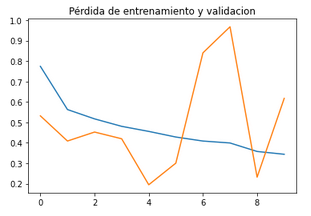
\includegraphics[width=0.45\textwidth]{./imagenes/perdida.png}
        \end{figure} 

        \item Precisión 
        \begin{lstlisting}[language=Python]
        plt.plot(H.history['accuracy'])
        plt.plot(H.history['val_accuracy'])
        plt.title('Precision de entrenamiento y validacion')
        \end{lstlisting}

        \begin{figure}[ht]
            \centering
            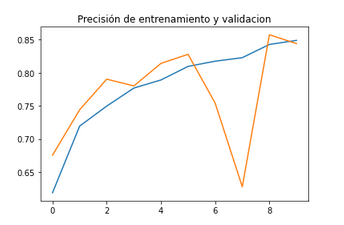
\includegraphics[width=0.5\textwidth]{./imagenes/precision.png}
        \end{figure} 
    \end{itemize}

    % Ejercicio 4.
    \item Salva tu modelo y súbelo.

    \textsc{Solución:} El modelo lo guardamos de la siguiente manera 
    \begin{lstlisting}[language=Python]
    model.save('mi_modelo.h5')
    \end{lstlisting}

    % Ejercicio 5.
    \item Úsalo para reconocer las $4$ imágenes anexas.
    
    \textsc{Solución:} Realizamos el reconocimiento de cada una de las cuatro 
    imágenes solicitadas.
    \begin{itemize}
        % Imagen 1.
        \item \textit{cat1.jpeg}
        \begin{lstlisting}[language=Python]
        from PIL import Image

        # Definimos los dos resultados posibles.
        categoria_final = {0:'gatito', 1:'perrito'}

        # Cargamos la imagen y la modificamos para poder hacer el 
        # reconocimiento.
        imagen1 = Image.open("imagenes/cat1.jpeg")
        imagen1 = imagen1.resize((128, 128))
        imagen1 = np.expand_dims(imagen1, axis = 0)
        imagen1 = np.array(imagen1)
        imagen1 = imagen1 / 255

        # Realizamos la prediccion.
        reconocimiento = model.predict_classes([imagen1])[0]

        # Visualizamos el resultado de la prediccion.
        print(reconocimiento, categoria_final[reconocimiento])
        \end{lstlisting}

        \begin{verbatim}
            0 gatito
        \end{verbatim}

        \begin{figure}[ht]
            \centering
            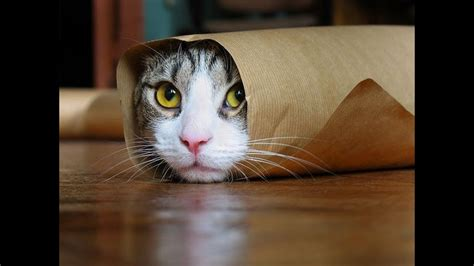
\includegraphics[width=0.4\textwidth]{./src/imagenes/cat1.jpeg}
        \end{figure} 

        % Imagen 2.
        \newpage
        \item \textit{cat2.jpg}
        \begin{lstlisting}[language=Python]
        # Cargamos la imagen y la modificamos para poder hacer el 
        # reconocimiento.
        imagen2 = Image.open("imagenes/cat2.jpg")
        imagen2 = imagen2.resize((128, 128))
        imagen2 = np.expand_dims(imagen2, axis = 0)
        imagen2 = np.array(imagen2)
        imagen2 = imagen2 / 255

        # Realizamos la prediccion.
        reconocimiento = model.predict_classes([imagen2])[0]

        # Visualizamos el resultado de la prediccion.
        print(reconocimiento, categoria_final[reconocimiento])
        \end{lstlisting}

        \begin{verbatim}
            0 gatito 
        \end{verbatim}

        \begin{figure}[ht]
            \centering
            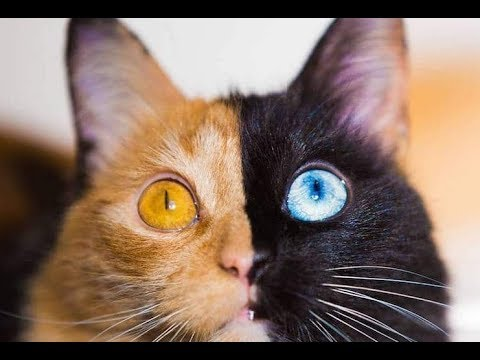
\includegraphics[width=0.35\textwidth]{./src/imagenes/cat2.jpg}
        \end{figure} 

        % Imagen 3.
        \item \textit{dog1.jpeg}
        \begin{lstlisting}[language=Python]
        # Cargamos la imagen y la modificamos para poder hacer el 
        # reconocimiento.
        imagen3 = Image.open("imagenes/dog1.jpeg")
        imagen3 = imagen3.resize((128, 128))
        imagen3 = np.expand_dims(imagen3, axis = 0)
        imagen3 = np.array(imagen3)
        imagen3 = imagen3 / 255

        # Realizamos la prediccion.
        reconocimiento = model.predict_classes([imagen3])[0]

        # Visualizamos el resultado de la prediccion.
        print(reconocimiento, categoria_final[reconocimiento])
        \end{lstlisting}

        \begin{verbatim}
            1 perrito
        \end{verbatim}

        \begin{figure}[ht]
            \centering
            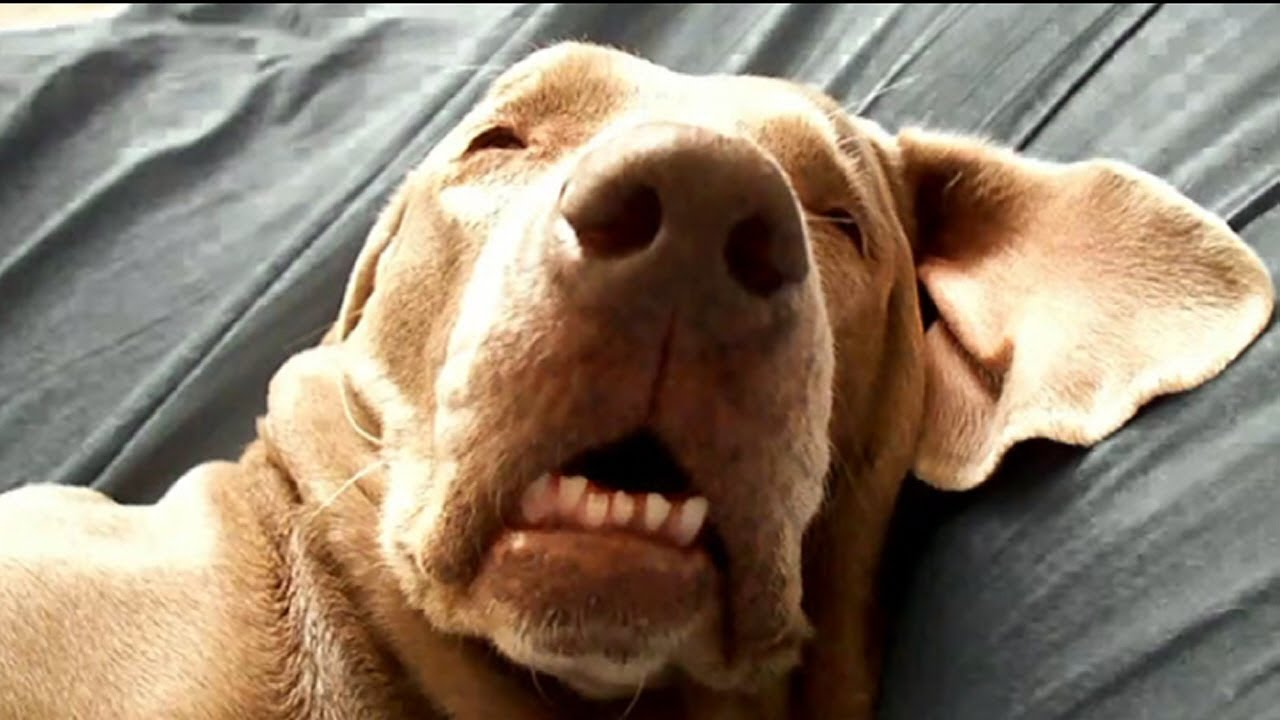
\includegraphics[width=0.4\textwidth]{./src/imagenes/dog1.jpeg}
        \end{figure} 

        % Imagen 4.
        \item \textit{dog2.jpeg}
        \begin{lstlisting}[language=Python]
        # Cargamos la imagen y la modificamos para poder hacer el 
        # reconocimiento.
        imagen4 = Image.open("imagenes/dog2.jpeg")
        imagen4 = imagen4.resize((128, 128))
        imagen4 = np.expand_dims(imagen4, axis = 0)
        imagen4 = np.array(imagen4)
        imagen4 = imagen4 / 255

        # Realizamos la prediccion.
        reconocimiento = model.predict_classes([imagen4])[0]

        # Visualizamos el resultado de la prediccion.
        print(reconocimiento, categoria_final[reconocimiento])
        \end{lstlisting}

        \begin{verbatim}
            1 perrito 
        \end{verbatim}

        \begin{figure}[ht]
            \centering
            
\includegraphics[width=0.4\textwidth]{./src/imagenes/dog2.jpeg}
        \end{figure} 
    \end{itemize}
\end{enumerate}
\end{document}
